




\section[Stats eg's]{Basic Statistics Examples}

\hidenum
\begin{frame}[noframenumbering]
\frametitle{Contents}
 \tableofcontents[currentsection,hideothersubsections,sectionstyle=show/hide]
\end{frame}
\shownum


\subsection{pbdMPI Example: Monte Carlo Simulation}

\begin{frame}[shrink]
  \begin{block}{Example \countex :  Monte Carlo Simulation}\pause
  Sample $N$ uniform observations $(x_i, y_i)$ in the unit square $[0, 1]\times [0,1]$.  Then
\begin{equation*}
\pi \approx 4\left(\frac{\#\ Inside\ Circle}{\#\ Total}\right) = 4\left(\frac{\text{\color{blue}{\# Blue}}}{\text{\color{blue}{\# Blue}}+\text{\color{red}{\# Red}}}\right)
\label{eqn:pi}
\end{equation*}
  \begin{center}
   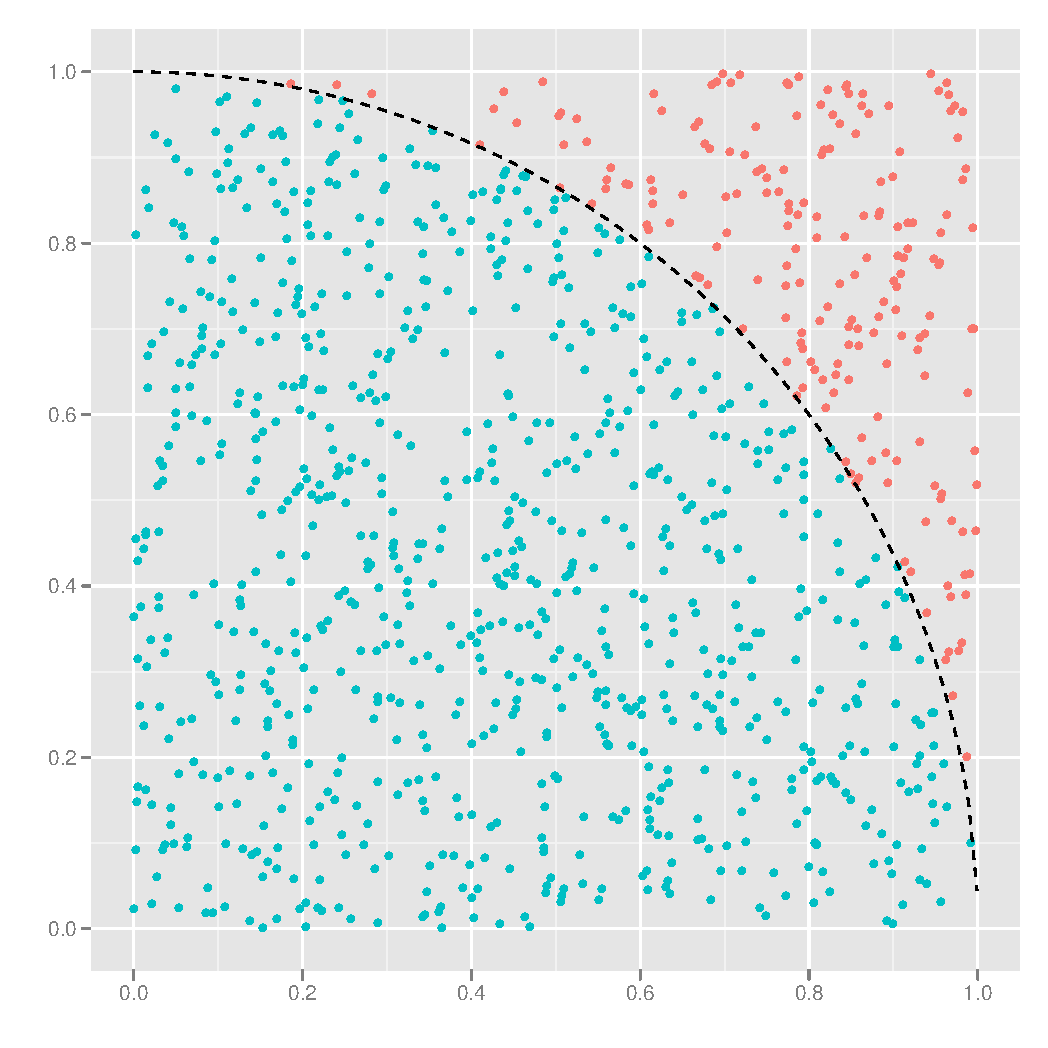
\includegraphics[scale=.25]{pics/pi} 
  \end{center}
  \end{block}
\end{frame}


\begin{frame}[fragile]
  \begin{block}{Example \showex :  Monte Carlo Simulation GBD Algorithm}\pause
    \begin{enumerate}
     \item Let $n$ be big-ish; we'll take $n=50,000$.
     \item Generate an $n\times 2$ matrix $x$ of standard uniform observations.
     \item Count the number of rows satisfying $x^2 + y^2 \leq 1$
     \item Ask everyone else what their answer is; sum it all up.
     \item Take this new answer, multiply by 4 and divide by $n$
     \item If my rank is 0, print the result.
    \end{enumerate}
  \end{block}
\end{frame}


\begin{frame}[fragile,scale,shrink]
  \begin{exampleblock}{Example \showex :  Monte Carlo Simulation Code}\pause
\begin{lstlisting}[title=Serial Code]
N <- 50000
X <- matrix(runif(N * 2), ncol=2)
r <- sum(rowSums(X^2) <= 1)
PI <- 4*r/N
print(PI)
\end{lstlisting}

\begin{lstlisting}[title=Parallel Code]
library(pbdMPI, quiet = TRUE)
init()
comm.set.seed(diff=TRUE)

N.gbd <- 50000 / comm.size()
X.gbd <- matrix(runif(N.gbd * 2), ncol = 2)
r.gbd <- sum(rowSums(X.gbd^2) <= 1)
r <- allreduce(r.gbd)
PI <- 4*r/(N.gbd * comm.size())
comm.print(PI)

finalize()
\end{lstlisting}
  \end{exampleblock}
\end{frame}

\begin{frame}[fragile]
  \begin{block}{Note}\pause
    For the remainder, we will exclude loading, init, and finalize calls.
  \end{block}
\end{frame}










\subsection{pbdMPI Example: Sample Covariance}

\begin{frame}
  \begin{block}{Example \countex :  Sample Covariance}\pause
  \begin{align*}
    cov(x_{n\times p}) = \frac{1}{n-1}\sum_{i=1}^n\left(x_i-\mu_x\right)\left(x_i-\mu_x\right)^T
  \end{align*}
  \end{block}
\end{frame}


\begin{frame}
  \begin{block}{Example \showex :  Sample Covariance GBD Algorithm}\pause
    \begin{enumerate}
     \item Determine the total number of rows $N$.
     \item Compute the vector of column means of the full matrix.
     \item Subtract each column's mean from that column's entries in each local matrix.
     \item Compute the crossproduct locally and reduce.
     \item Divide by $N-1$.
    \end{enumerate}
  \end{block}
\end{frame}


\begin{frame}[fragile,shrink]
  \begin{exampleblock}{Example \showex :  Sample Covariance Code}\pause
\begin{lstlisting}[title=Serial Code]
N <- nrow(X)
mu <- colSums(X) / N

X <- sweep(X, STATS=mu, MARGIN=2)
Cov.X <- crossprod(X) / (N-1)

print(Cov.X)
\end{lstlisting}
  
\begin{lstlisting}[title=Parallel Code]
N <- allreduce(nrow(X.gbd), op="sum")
mu <- allreduce(colSums(X.gbd) / N, op="sum")

X.gbd <- sweep(X.gbd, STATS=mu, MARGIN=2)
Cov.X <- allreduce(crossprod(X.gbd), op="sum") / (N-1)

comm.print(Cov.X)
\end{lstlisting}
  \end{exampleblock}
\end{frame}







\subsection{pbdMPI Example: Linear Regression}

\begin{frame}
  \begin{block}{Example \countex :  Linear Regression}\pause
      Find $\bbeta$ such that
      \begin{align*}
      \by = \bX\bbeta + \bepsilon
      \end{align*}

      When $\bX$ is full rank,
      \begin{align*}
      \hat{\bbeta} = (\bX^T\bX)^{-1}\bX^T\by \label{math:ols}
      \end{align*}
  \end{block}
\end{frame}


\begin{frame}
  \begin{block}{Example \showex :  Linear Regression GBD Algorithm}\pause
    \begin{enumerate}
     \item Locally, compute $tx = x^T$
     \item Locally, compute $A = tx * x$. Query every other processor for this result and sum up all the results.
     \item Locally, compute $B = tx * y$.  Query every other processor for this result and sum up all the results.
     \item Locally, compute $A^{-1} * B$
    \end{enumerate}
  \end{block}
\end{frame}


\begin{frame}[fragile,shrink]
  \begin{exampleblock}{Example \showex :  Linear Regression Code}\pause
\begin{lstlisting}[title=Serial Code]
tX <- t(X)
A <- tX %*% X
B <- tX %*% y

ols <- solve(A) %*% B
\end{lstlisting}
  
\begin{lstlisting}[title=Parallel Code]
tX.gbd <- t(X.gbd)
A <- allreduce(tX.gbd %*% X.gbd, op = "sum")
B <- allreduce(tX.gbd %*% y.gbd, op = "sum")

ols <- solve(A) %*% B
\end{lstlisting}
  \end{exampleblock}
\end{frame}